\section{Theoretical background}
\label{sec:theory}
\todo{add theory intro}

\subsection{Ozone chemistry and \ch{NO} to \ch{NO2} conversion}
\label{sec:chemistry}

This section lays the chemical groundwork for the construction of our
\ch{NO} to \ch{NO2} converter. First we will introduce the rate
coefficient to get a measure for the speed of a
reaction. Afterwards we will have a look at possible ways to generate
Ozone out of ambient air and then describe Ozone induced reactions
concerning Nitrogenoxides. This section is mainly inspired by and
taken from~\cite{bsc}.

\subsubsection{The rate coefficient}
\label{sec:rate}

During our conversion we will have many chemical reactions of the form

\begin{align*}
  \ch{A + B -> C + D}.
\end{align*}

Some of them will have positive, wanted effects, others describe side
effects and we want to suppress them as much as possible. However we
have only two parameters we can adjust. The first is the Ozone
concentration, which we can vary slighty and very roughly and the
other one is the reaction pathlength and.  Thus our best chance to
select certain reactions is to set ther reaction time to a value that
corresponds to the different reaction speeds of the equations, making
sure that wanted reactions have enough time to happen while
simultaneously suppressing unwanted reactions. Of
course this is only possible, if the wanted reactions run faster than
the unwanted ones.

With this motivation in mind, we need a measure for the reaction
speed. Thinking of speed in this setting means to think of change of
compound concentration. In this section we will use $c$ to denote
concentrations. Using the above mentioned prototypic equation, we can
see that the change of concentration, i.\,e. $\dot c$, of the
different species are related by:
\begin{align*}
  -\dot c(A) = - \dot c(B) = \dot c(C) = \dot c(D).
\end{align*}

Next we need a relation between these derivatives and the educt
concentrations. The probability for a reaction to take place should be
proportional both to $c(A)$ and $c(B)$ as the two particles need to
`meet'. Thus we expect
\begin{align}
  -\dot c(A) = - \dot c(B) = k \cdot c(A) \cdot c(B), \label{eq:rate}
\end{align}

where the proportionality constant $k$ ist called \emph{rate
  coefficient}. It is often given in units of
\si{\hertz\per\cubic\centi\meter}. This $k$ is our desired reaction
speed measure, as it describes the
reaction time concentration independently.

In our case the Ozone concentration will often far exceed the
concentration of the other trace gases. This allows us to think of its
concentration as approximately constant. If we set $c(B)$ constant in
Equation~\eqref{eq:rate}, then we get a well known ordinary first
order differential equation with solution
\begin{align*}
  c(A,t) = c(A,0)\exp(-kc(B)\cdot t).
\end{align*}

In this limiting case we see that the decay time is given by $\tau =
(kc(B))^{-1}$, making the connection of $k$ to the reaction speed
obvious.

\subsubsection{Ozone generation}
\label{sec:theory-ozone}

In this section we will discuss the generation of Ozone (\ch{O3}) out of ambient
air. The main idea comes from the observation that stratospheric
\ch{O3} protects us from ultraviolet (UV) light. Thus Ozone needs to
have absorption bands there. Furthermore normally the Ozone layer is
not depleted, but regenerates itself, so there needs to be a reaction
cycle building Ozone out of ordinary Oxygen molecules (\ch{O2}).

The following equations describe the Ozone-Oxygen cycle in the
atmosphere.  The cycle is often referred to as \emph{Chapman-Cycle}
due to its first investigator (c.\,f.~\cite{chapman}
and~\cite{roedel}). We will see that we can use these atmospheric
reactions to generate Ozone in the laboratory. In some of the
reactions an additional molecule is necessary to assure momentum
conservation. This inert reaction participant is always denoted
\ch{M}.

The first part of the cycle contains the reactions, that generate
\ch{O3} out of \ch{O2}

\begin{align}
  \ch{O2} + h\nu &\ch{-> 2 O(^3P)},\nonumber\\
  \ch{O(^3 P) + O2 + M} &\ch{-> O3 + M}. \label{eq:ozone}
\end{align}

We see that a photon splits an Oxygen molecule and the excited
Oxygen atom reacts with another \ch{O2} molecule to form Ozone. For
the first reaction to take place we need a photon of the wavelength
$\lambda = \SI{184.9}{\nano\meter}$.

The next part of the cycle shows, how another UV photon ($\lambda =
\SI{253.6}{\nano\meter}$) can destroy
Ozone and create a ground state Oxygen atom. This Oxygen atom will
then be reexcited:

\begin{align}
  \ch{O3} + h\nu \ch{&-> O(^1 D) +
  O2}, \label{eq:split}\\
  \ch{O(^1 D) + M & -> O(^3 P) + M}.\nonumber
\end{align}

After this reaction there are two possible reaction paths. First the $\ch{O}(^3
P)$ can reenter into Equation~\eqref{eq:ozone}, such that there is no
net change in Ozone or it could react to form \ch{O2} by the
following mechanisms

\begin{align*}
  \ch{2 O(^3 P) + M & -> O2 + M} \quad \text{and}\\
  \ch{O(^3 P) + O3 & -> 2 O2},
\end{align*}
leading to a net loss of Ozone. 

Introducing a UV light source with
an intensity peak at $\lambda = \SI{184.9}{\nano\meter}$
will start the above cycle. In our case we use a Mercury lamp, which
also has a peak at $\lambda = \SI{254}{\nano\meter}$. So the
Chapman-Cycle will enter an equilibrium state with a constant Ozone
Oxygen ratio. The value of this ratio depends on the
intensity ratio at the two wavelengths mentioned above. Since the
main energy output of the lamp is at \SI{254}{\nano\meter}, the ratio
will be small. However, there is around \SI{20}{\%} Oxygen in ambient
air, sucht that in absolute terms we will still produce an Ozone
surplus. The expected Ozone value can be computed exactly and has been
done so in~\cite{bsc}. Using this specific lamp leads to a value of
$c(\ch{O3}) = \SI{300}{ppm}$. Of course this value will vary for
different currents, but since we are not intersted in the exact value,
only in the order of magnitude, this estimation will suffice for our
purpose. The experimentally verified output of our generator can be
found in Section~\ref{sec:ozone}.

\subsubsection{Ozone triggerd Nitrogenoxide reactions}
\label{sec:o-no}

In this section we will have a look at all reactions concerning
chemicals consisting of Nitrogen and Oxygen. Our aim is to achieve a
complete conversion of the Nitrogen Monoxide (\ch{NO}) to Nitrogen
Dioxide (\ch{NO2}). However, introducing Ozone to the sample air
triggers further reactions. If these lead to a net change of \ch{NO2}
we have additional effects to correct. All reactions are given with
their corresponding rate coefficient $k$ which were taken
from~\cite{bsc}. In Section~\ref{sec:requirements} we will discuss the
implications of the reactions here on the setup of our converter.

Our desired reaction is the following

\begin{align}
  \ch{NO + O3 & ->[$k=\SI{1.8e-14}{\hertz\per\cubic\centi\meter}$] NO2
                + O2}. \label{eq:no}
\end{align}

If this were the only reaction, we would have a one to one conversion
from \ch{NO} to \ch{NO2}. With enough Ozone our problem would be
solved. However, this is not the only reaction taking
place. Nitrogen Dioxide itself can be oxidized by Ozone to generate
Nitrogen Trioxide (\ch{NO3}):

\begin{align}
  \ch{NO2 + O3 ->[$k=\SI{3.5e-17}{\hertz\per\cubic\centi\meter}$] NO3
  + O2}. \label{eq:no2}
\end{align}

Luckily, we see that the rate coefficients of the two reactions are
very different and the first one is approximately three orders of
magnitude larger than the second one. Additionally there is a very
fast reaction of \ch{NO3} with \ch{NO}

\begin{align}
  \ch{NO + NO3 ->[$k=\SI{6.9e-2}{\hertz\per\cubic\centi\meter}$] 2 NO2},\label{eq:back}
\end{align}

such that small Nitrogen Trioxide concentrations should decay
quickly. If we assume no \ch{NO3} in our sample air (which is sensible
for day time measurements) Equation~\eqref{eq:back} should guarantee
that the oxidation of \ch{NO2} should be compensated. 

Sadly, this is not the only reaction using \ch{NO3}. Some can react
with \ch{NO2} to generate the solid \ch{N2O5}

\begin{align}
  \ch{NO2 + NO3 + M
  <=>[$k=\SI{1.9e-12}{\hertz\per\cubic\centi\meter}$][$k=\SI{2.6e-11}{\hertz\per\cubic\centi\meter}$]
  N2O5 + M}. \label{eq:laughing}
\end{align}

As we can see the equilibrium of Equation~\eqref{eq:laughing} lies on the
side of the educts, so the effect should not be too large. Especially
if the \ch{NO3} concentrations are small. Still in the further
analysis we will try to allow enough time for Reaction~\eqref{eq:no}
to take place, while being too fast for Reaction~\eqref{eq:no2}. Such
that we can simply ignore the reaction paths for \ch{NO3}.

\subsection{Basics of fluid dynamics}
\label{sec:fluid}

One important aspect of this work consists in the understanding of the
different gas flows in the instrument. We need an estimate for the
mixing time of Ozone with the sample air and then we need to know how
long our mixing and reaction pathlength needs to be in order to
achieve a full conversion. These questions can all be answered using a
few basic principles from fluid dynamics. First we will have a look at
laminar flows in cylindric vessels (in our case tubes) to get a
connection between the flow and the maximum speed in the tube. Next we
have a look at diffusion of gases. As we only have laminar flows,
diffusion is the only way mixing can take place, so we need an
estimate of the time this mixing takes. Lastly we will discuss
adsorption of some trace gases at teflon, silica gel and activated
carbon to better our understanding of the filtering effects in the
instrument. 

\subsubsection{Laminar flows in cylinders}
\label{sec:cylinder}

We are interested in what regime the gas transport in the tube
settles. Especially after the Ozone enriched air is added to the
sample air, we would benefit from ab turbulent flow in the system as
it would ensure a faster mixing of the gases. To see whether we have
a laminar or a turbulent flow, we use the phenomenological \emph{Reynold's
number}

\begin{align*}
  \operatorname{Re} = \frac{\rho \cdot d \cdot \bar v}{\eta},
\end{align*}

where $\rho$ denotes the density of our gas, $d$ is a characteristc
length of the system, in our case the tube diameter, $\bar v$ is the
average velocity of the gas and $\eta$ its viscosity. As a rule of
thumb the flow in a cylinder will be laminar, if the Reynold's number
is smaller than the critical Reynold's number
$\operatorname{Re}_{\text{c}} = 2300$ and it will be turbulent if the
number is higher than $3000$ (c.\,f.~\cite{maschbau}). In our system
we have $d = \SI{4}{\milli\meter}$, $\rho \approx
\SI{1.2}{\kilo\gram\per\cubic\meter}$ and $\eta \approx
\SI{17.1}{\micro\pascal\second}$(c.\,f.~\cite{maschbau}). Furthermore
we work with a flow of $\Phi = \SI{2}{\liter\per\minute}$. With the
above diameter this leads to an average velocity of $\bar v =
\SI{2.7}{\meter\per\second}$. Using this data we compute the Reynold's
number to be

\begin{align*}
  \operatorname{Re} \approx 760 < 2300.
\end{align*}

Thus we see that we work solely in the laminar setting and we need to
understand the velocity distribution in this case in order to allow
enough time for mixing and the chemical reactions to take place. The
law behind the flow in a cylindric tube is called
\emph{Hagen-Poiseulle} and we follow the exposition used
in~\cite{gerthsen} to derive it.

Denote by $r_0$ the inner radius of our tube and by $l$ its length. We
assume that we are in the equilibrium state, such that all forces need
to add to zero. We look at a cylinder with radius $0 \leq r \leq
r_0$. To have a nonzero flow, we need a pressure difference at the two
ends of the tube denoted $\Delta p$. The force exerted on the cylinder
by the pressure is given by
\begin{align*}
  F_b = - \pi r^2 \Delta p,
\end{align*}

where the minus sign is introduced because the force points in the
opposite direction of the pressure gradient. At the boundary of our
cylinder we have to consider friction between the adjoining layers of
fluid. The force exerted by it is proportional to the area of
friction, i.\,e.\ the cylinder barrel and to the difference in velocity
between the fluid within the cylinder and without, since we have to
look at an infinitesimal anulus around the boundary, we get a
proportionality to the velocity gradient $\frac{\d[v]}{\d[r]}$. Thus
the force of friction takes the form

\begin{align*}
  F_f = \eta \cdot 2\pi r \cdot l \cdot \frac{\d[v]}{\d[r]}.
\end{align*}

We are at an equilibrium state, thus we need $F_b = F_f$ for all
possible $r$ to hold. This leads us to the following differential
equation for the velocity

\begin{align*}
  \frac{\d[v]}{\d[r]} = - \frac{\Delta p}{2l\eta} \cdot r
\end{align*}
 
which can be directly integrated. Using the boundary condition $v(r_0)
= 0$, i.\,e.\ the fluid sticks to the wall of the tube, we yield

\begin{align}
  v(r) = v_0 \left ( 1 - \left( \frac{r}{r_0} \right)^2 \right) \quad
  \text{with }\ v_0 \coloneqq \frac{\Delta p r_0^2}{4 l \eta}. \label{eq:v}
\end{align}

This can be further integrated to yield the flow $\Phi$ of the system

\begin{align*}
  \Phi = \int_A v(r) \d[A] = 2\pi \int_0^{r_0} v(r)r \d[r] = \frac{\pi
  r_0^4}{8\eta l} \cdot \Delta p.
\end{align*}

This is the standard form of the Hagen-Poiseulle law. One remarkable
obersvation is that there is a power four law between the radius of
the tube and the flow. More interesting for us is the relation between
the average velocity $\bar v$ and the maximum velocity $v_0$ at the
center of the pipe

\begin{align*}
  \bar v = \frac{\Phi}{\pi r_0^2} = \frac{\Delta p r_0^2}{8\eta l} \stackrel{\eqref{eq:v}}{=} \frac{v_0}{2}.
\end{align*}

So we see that at the center the the velocity is twice as large as the
average. We need to keep this effect in mind when it comes to compute
the dwell time of our gases.

\subsubsection{Diffusion}
\label{sec:diffusion}

As was shown in the previous section, the gas flows laminarly through
our instrument. Thus the only mechanism by which gas mixing can occur
is \emph{diffusion}. Therefore we want an estimate for the time it
takes for diffusion to take place. This exposition drew inspiration
from~\cite{fluid}.

We are interested in the evolution of the concentration $n$ of a
species. Fick's first law states that the flow $\Phi$ of the species
is proprotional to the concentration gradient $\nabla n$ and that the
species flows from higher to lower concentration. We yield

\begin{align*}
  \Phi = - D \nabla n,
\end{align*}
where $D > 0$ is called the \emph{diffusion constant}. Assuming no
sources and sinks and using the continuity equation for fluids, we
arrive at Fick's second law

\begin{align*}
  \dot n = - \nabla \Phi = \nabla (D \nabla n) = D \cdot \Delta n,
\end{align*}
where for the last equation we assumed and istotrope medium, i.\,e.\
$\nabla D = 0$. This is a second order linear partial differential
equation and for arbitrary boundary conditions it can become
arbitrarily hard to solve. Since we are mostly interested in the
diffusion of species at small time scales, we can assume our vessel
inifinitely large. With this the equation becomes accessible via
Fourieranalysis. Let

\begin{align*}
  \hat n(k,t) = \mathcal{F}[n](k,t)
\end{align*}
be the fouriertransform of $n$ with regard to the three spatial
coordinates $x$. Using the known relation $\mathcal{F}[\partial_{x_j}
n](k,t) = -ik_j \hat n(k,t)$, we can transform the equation to

\begin{align*}
  \partial_t \hat n(k,t) =  - Dk^2 \hat n(k,t)
\end{align*}

a linar first order ordinary differential equation, with the well
known solution

\begin{align}
  \hat n(k,t) = c(k) \cdot \exp(-Dk^2 t). \label{eq:sol-ft}
\end{align}

To determine $c(k)$, we need to introduce an initial value. We again
work with an idealistic, simplified model. We will later on be
interested in the diffusion of one molecule. Therefore we work with
the initial condition
\begin{align*}
  n(x,0) = n_0 \delta(x),
\end{align*}
i.\,e.\ all the species (or for $n_0 = 1$: the particle) is localized
at one point for $t = 0$. We can fouriertransform this initial
condition, too, and yield

\begin{align*}
  \hat n(k,0) = n_0.
\end{align*}
Plugging this into Equation~\eqref{eq:sol-ft}, we get

\begin{align*}
  \hat n(k,t) = n_0 \exp(-Dt \cdot k^2).
\end{align*}
This is a Gaußian function with regard to the variable $k$. If we want
the solution of the diffusion equation in terms of $x$ we need to
compute the inverse Fourier transform of $\hat n$. However, we know
that the Gauß function is an Eigenfunction of the Fouriertransform
(and its invers). Additionally the total concentration needs to be the
same for all times $t$. Thus we yield

\begin{align*}
  n(x,t) = \frac{n_0}{(2\pi \cdot 2Dt)^{3/2}} \cdot \exp \left(
  -\frac{1}{2} \cdot \frac{x^2}{2Dt} \right).
\end{align*}
This is the desired solution. This allows us to describe the statistic
behaviour of a particle undergoing diffusion. Setting $n_0 = 1$, we
arrive at the probability distribution for the particle, which is just
a Gaußian distribution with a timedependent variance. We see that the
expectation value of the position $\langle x \rangle$ is always
0. However the standard deviation $\sigma = \sqrt{2Dt}$ grows larger
over time, such that for the \emph{mean squared displacement}, we
yield the following relation

\begin{align}
  \langle x^2 \rangle = \sum_{j=1}^3 \langle
  x_j^2 \rangle = \sum_{j=1}^3 \sigma^2 = 3 \cdot 2Dt, \label{eq:mqd}
\end{align}

where we used $\langle x \rangle = 0$. This mean squared displacement
can now be used as a measure to gauge the distance travelled by a
molecule. We will apply it to gauge the time needed for a new gas
species (in our case Ozone) to fill a volume sufficiently for the
chemical reactions to take place.

\subsubsection{Adsorption}
\label{sec:adsorption}
\todo{find something out and write something about adsorption}

\subsection{Technical requirements for the converter}
\label{sec:requirements}

The above considerations lead to some technical requirements in the
construction of our converter. First and obviously we need to use well
filtered air in the Ozone generator as not to introduce other trace
gases which would disturb the measurement. The normal procedure
consists of using an activated charcoal, a silica gel and a particle
filter. However, some Nitrogen derivates\todo{which ones? What reactions?} pass all these
filters. Normally this is of no concern, as they have a zero
absorption cross section in our wavelength range. In the case of our
Ozone generator the molecules will react and form additional \ch{NO2},
which will distort our measured signals. Thus we need to introduce
another filter after the Ozone generator, which should be transparent
for Ozone, but impervious to \ch{NO2}. Luckily a Silica gel filter
suffices these constraints. At first it filters Ozone as well as
\ch{NO2}, but the saturation level for Ozone is far lower for Ozone,
such that it will pass unhindered, while the Nitrogen Dioxide is kept
back. For the filtering to be effective, we also need to introduce a
reaction path between the Ozone generation chamber and the Silica gel
filter for the conversion to \ch{NO2} to be completed.

The next restriction is that we need a nigh \SI{100}{\%} conversion of
\ch{NO} to \ch{NO2}. This leads to three considerations. Firstly, we
need enough time for the mixing of the ozone with the sample air to
take place. Secondly, we need enough time for the actual reaction to
take place. Thirdly, we need the time to be short enough, such that we
do not loose to much \ch{NO2} to further oxidation.

Concering our first consideration, we have to look at
Section~\ref{sec:fluid} to estimate the mixing time. As we work with
laminar flows in the reaction path (c.\,f.\ Sec.~\ref{sec:cylinder}),
the mixing will be dominated by diffusion. Thus we use the mean
squared displacement to estimate the time the Ozone takes to cross the
tube diameter. In our case we use tubes with $d =
\SI{4}{\milli\meter}$ and the diffusion constant for Ozone in air was
taken to be $D = \SI{0.137}{\square\centi\meter\per\second}$ (at $T =
\SI{298}{\kelvin}$ and $p = \SI{1}{\text{bar}}$
c.\,f.~\cite{diff-ozone}). With these values we get
\begin{align*}
  t_{\text{mix}} = \frac{d^2}{6\cdot D} = \SI{0.195}{\second}
\end{align*}

Turning towards considerations two and three, we need to gauge the
reaction times. For this we have to set a desired conversion
ratio. For our estimates we work with a ratio of \SI{99}{\%}. 
Since the Ozone generator will supply an
overabundance of \ch{O3}, we can use the linear ordinary
differential equation approximation introduced in
Section~\ref{sec:rate}. Thus the conversion ratio is
given by
\begin{align*}
  \exp(-kc(\ch{O3})\cdot t),
\end{align*}
where $t$ is the reaction time. $1$ stands for no
conversion at all (i.\,e.\ no decrease in the educt concentration) and
$0$ stands for complete conversion. For \SI{99}{\%} we need
\begin{align}
  kc(\ch{O3}) \cdot t_{\text{react}} \gtrsim 4.6. \label{eq:react-bound}
\end{align}
As a lower bound for the Ozone concentration we use
\begin{align*}
  c(\ch{O3}) = \SI{2}{ppm} = \SI{4.996e13}{\per\cubic\centi\meter} 
\end{align*}
and using $k = \SI{1.8e-14}{\hertz\per\cubic\centi\meter}$, we yield
the following natural time scale
\begin{align*}
  \tau^{-1} & = k c(\ch{O3}) = \SI{0.90}{\hertz}.
\end{align*}

Together with Equation~\eqref{eq:react-bound} this leads to

\begin{align*}
  t_{\text{react}} \gtrsim \SI{5.1}{\second}.
\end{align*}

Using $t_{\text{react}}$ to compute the conversion ratio of
$\ch{NO2}$ to $\ch{NO3}$, we get \SI{0.9}{\%}. So with this reaction
time we should expect about a \SI{2}{\%} error in the retrieved
\ch{NO} concentration. Hopefully, the results will be better than
that, as some of the produced \ch{NO3} will (as described in
Section~\ref{sec:o-no}) quickly degrade to \ch{NO2} and the Ozone
concentration is likely to be underestimated.

As a last step we want to translate the needed mixing and reaction
time
\begin{align*}
  t = t_{\text{mix}} + t_{\text{react}} = \SI{5.3}{\second}
\end{align*}
to its associated pathlength. Using the applied flow
of $\Phi = \SI{2}{\liter\per\minute}$, we can compute the average
speed of the gas to be
\begin{align*}
  \bar v = \frac{\Phi}{\pi r^2} = \SI{2.7}{\meter\per\second}. 
\end{align*}
As was described in Section~\ref{sec:cylinder} this corresponds to a
maximum speed at the center of the tube of

\begin{align*}
  v_0 = 2\cdot \bar v = \SI{5.4}{\meter\per\second}.
\end{align*}

Using these two speeds we get

\begin{align*}
  \bar l & = \SI{14.31}{\meter} \quad \text{and}\\
  l_0 & = \SI{28.62}{\meter}
\end{align*}
as our pathlengths.

For the experiment we oriented at $\bar l$, as the maximum speed is
only relevant for a rather small cross section of the
cylinder. Most experiments were performed at $l = \SI{10}{\meter}$,
such that part of the conversion reaction was taking place inside the
cavity. The idea behind this is to have the conversion peak close to
the center of the cavity as this should lead to the best conversion
ratio averaged over all the cavity.

\subsection{The physics behind CE-DOAS}
\label{sec:ce-doas-physics}

In the following sections we will discuss the physical concepts
necessary to understand the Cavity Enhance Diffirential Absorption
Spectroscopy (CE-DOAS). First, we will investigate the Lambert-Beer
Law. This leads directly to the so called \emph{Longpath}-DOAS
instrument. As the name already indicates, those need a long
lightpath, since normally the absorption cross sections are very
small. Hence lastly we introduce the \emph{cavity enhancement} to
overcome this restriction.

The presentation follows mostly~\cite{fp58} with a few inspirations
taken from~\cite{bsc} and~\cite{platt}.

\subsubsection{The Lambert-Beer Law}
\label{sec:lambert-beer}

The \emph{Lambert-Beer Law} ist the underlying principle behind the
main measurement method used in this work. It concerns itself with the
evolution of the light intensity $I_0$ which propagates a certain
distance $L$ through air. It assumes an exponential decay over $L$, so
we can write

\begin{align}
  I(\lambda, L) = I_0(\lambda) \cdot \exp[-\epsilon(\lambda) \cdot
  L], \label{eq:lb-easy}
\end{align}

where $\epsilon$ is called \emph{absorption coefficient}. This
coefficient contains all the influences of the matter on the
absorption behaviour and can thus be split to account for the different
absorption and scattering mechanisms:

\begin{align*}
  \epsilon = \epsilon_a + \epsilon_R + \epsilon_M,
\end{align*}

where $\epsilon_a$ denotes the absorption and scattering due to the
trace gases, $\epsilon_R$ denotes Rayleigh scattering and $\epsilon_M$
Mie scattering. Next we want to understand the influence of the trace
gases on $\epsilon_a$ a little better. The absorption should be
proportional to the concentration of the gases, so we write

\begin{align}
  \epsilon_a(\lambda) = \sum_{i=1}^n \sigma_i(\lambda) \cdot \bar c_i, \label{eq:lb-abs}
\end{align}

where $i$ sums over all the trace gases present in the penetrated
air, $\bar c_i$ is the associated average concentration and $\sigma_i$
is calld \emph{absorption cross section}. For the above formula to be
useful to determine the concentration of our trace gases, we need to
have a very homogenous air sample, so that we can assume that the
concentration within it is constant. As we will see this assumption is
sensible for CE-DOAS, if one works with Longpath-DOAS measurements one
has to work with other parameters, e.\,g.\ the collon density.

Equations~\eqref{eq:lb-easy} and~\eqref{eq:lb-abs} now contain the central idea for our
spectroscopic method. We can measure the intensity spectra $I$ and
$I_0$, we can also determine the pathlength $L$. If we now want to
compute the concentration of our trace gases, we only need the
absorption cross sections, which can be found in the
literature. Thus lastly we introduce the \emph{Optical
  Density} 

\begin{align*}
  D(\lambda) = \ln \left(\frac{I(\lambda)}{I_0(\lambda)}\right) = - L
  \cdot \sum_{i=1}^n \sigma_i(\lambda) c_i,
\end{align*}

which contains all the necessary information.

\subsubsection{The DOAS method}
\label{sec:doas}

Differential Optical Absorption Spectroscopy uses the Lambert-Beer Law
to compute the concentrations of trace gases in the air. There are a
few more technicalities we need to respect. First of all, we must have
a look at the absorption crosssections of different trace gases. If we
want to be able to discern different gases and even compute their
concentration, we need the crosssections to be sufficiently
separating.

\begin{figure}[htbp]
  \centering
  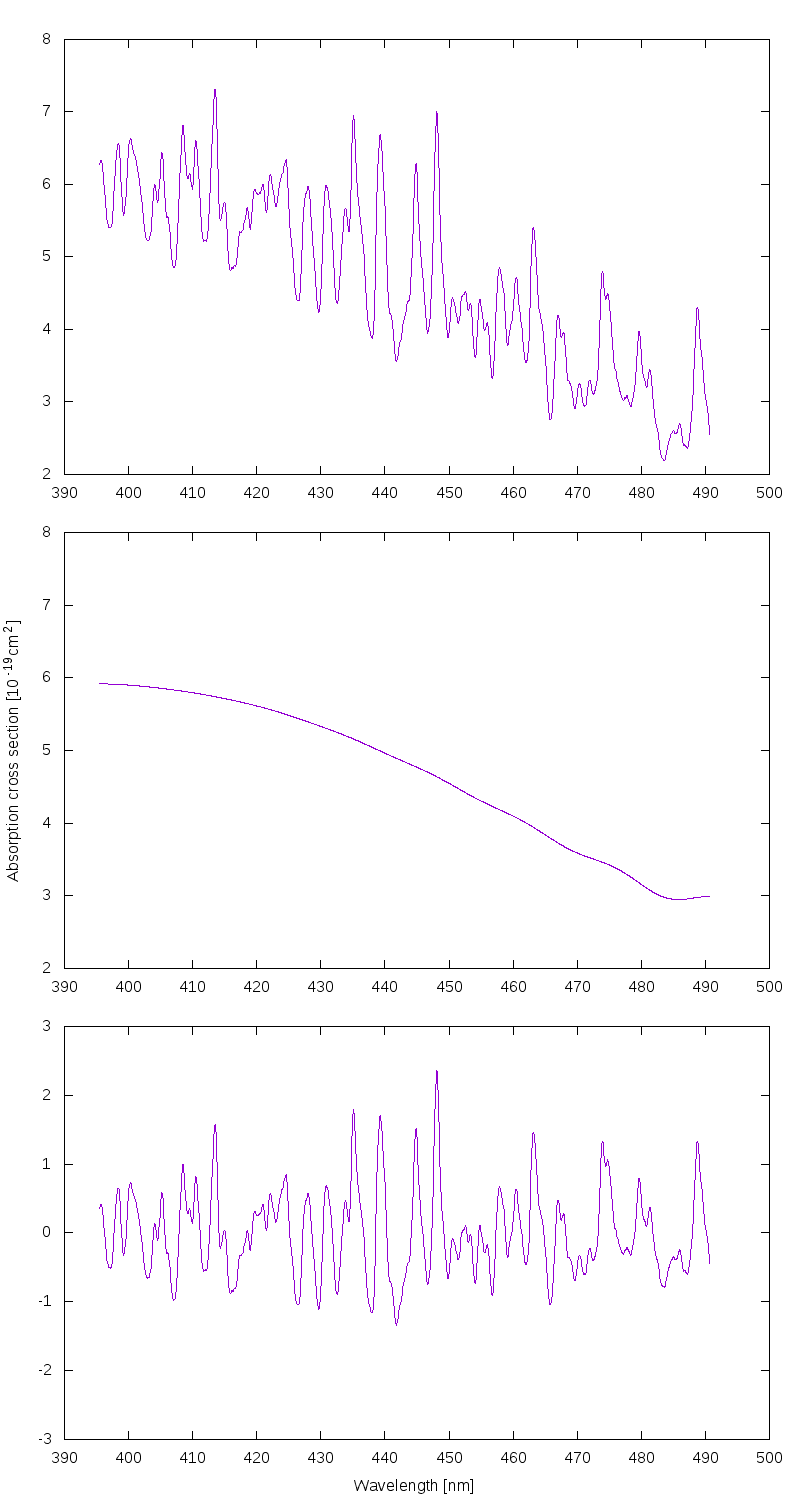
\includegraphics[width=0.7\textwidth]{NO2_conv.png}
  \caption{Absorption cross section of \ch{NO2} in the region around
    \SI{440}{\nano\meter}. From top to bottom we have the complete
    cross section $\sigma$, the broadband part $\sigma^b$ and the
    differential part $\sigma'$. The cross section is adapted to the
    resolution of the spectrograph used in the measurements
    (c.\,f.\ Sec.~\ref{sec:inclusion}).}
  \label{fig:no2-cross}
\end{figure}

As can be seen in Figure~\ref{fig:no2-cross}h the
cross sections can be separated into two parts: 

\begin{align*}
  \sigma = \sigma^b + \sigma'.
\end{align*}
One ($\sigma^b$) only weakly
wavelength dependent and a narrowband
structure ($\sigma'$) on top which differs strongly for different species. This
narrowband structure is what will allow us to discern the gases. It is
called the \emph{differential band}. Hence the name of the measurement
method. Putting what we used so far into the Lambert-Beer equation we
yield

\begin{align*}
  I(\lambda, L) & = I_0(\lambda) \exp \left ( \sum_{i=1}^n L \cdot
                  (\sigma^b_j(\lambda) + \sigma'_j(\lambda))\cdot c_j + L[\epsilon_R +
                  \epsilon_M]\right) \\
                & = I'_0(\lambda) \exp \left( \sum_{i=1}^n L \cdot
                  \sigma'_j(\lambda) \cdot c_j \right),
\end{align*}
where we collected all the broadband structure within $I'_0$. This
makes sense, as our $I_0$ spectrum often will not be free of the Rayleigh
and Mie scattering processes and thus are already taken into
account. Furthermore residual broadband structure can be handled in
the fitting process by adding a polynomial function. Thus we fit

\begin{align}
  f(\lambda) = - \sum_{i=1}^n c_i \cdot L \cdot \sigma'_i(\lambda) +
  \sum_k a_k \lambda^k \label{eq:doas-fit}
\end{align}
to the Optical Density, where the concentrations $c_i$ and the polynomial
coefficients $a_k$ are to be determined. The degree of the polynomial
is generally fixed to \num{4}.

One other technical aspect is how to adapt the literature
absorption cross sections to our spectrometer resolution. Some have
been computed theoretically others have been 
measured with a very high resolution. So we are given the
cross sections, however, we need to adapt them to the spectrometer used
in our measurement instrument, since it has a far lower
resolution. The effect of this lower resolution is that narrow
emission lines get smeared out. This smearing out is called
\emph{instrument function}. To determine it, we can measure the
spectrum of a Mercury lamp and use one of the
(normally very narrow) emission lines as a convolution kernel. The
narrow line is broadened and we can assume that all other used
measurements are broadened by the same amount. So if we convolute our
crosssections with this \ch{Hg} line, we will compensate for
the lower resolution. This step has to be done before the actual fit
and in Equation~\eqref{eq:doas-fit} the convoluted cross sections have
to be used.

This plain DOAS method is used as measurement method on
Section~\ref{sec:ozone-setup}. 

\subsubsection{The CE-DOAS method}
\label{sec:ce-doas}

Since the absorption coefficents $\epsilon$ are so small, we need a
very long pathlength $L$ to see a signal using the DOAS method. One
possibility is to really use a very long geometrical pathlength with
mirrors and telescopes. With this we are able to obtain pathlengths
between \num{1} and \SI{10}{\kilo\meter}~\cite{platt}. These so called
\emph{Longpath-DOAS} instruments have advantages, but also a few
disadvantages one of them clearly being that we need a lot of space
and in the process we average the concentration of our trace gases
over a large column.

An alternative approach is to increase the lightpath by the use of
optical instruments, i.\,e.\ mirrors. Using two highly reflective
mirrors we can obtain very large optical pathlengths, while still
having a managable geometrical pathlength. The price we pay by taking
this approach lies in the fact that now our pathlength becomes
wavelength dependent as this is true for the reflectivity of all
highly reflective mirrors. 

In this paragraph we will generalize the DOAS approach keeping in mind
that our pathlength is not constant anymore. On the way we try to
separate two effects on the pathlength. First the shortening due to
the absorption by the trace gases and secondly the influence by the
reflectivity.

The geometrical setup is the following:\todo{setup}

where we have two mirrors with reflectivity $R_i$, transmittance $T_i$
and absorption $A_i$. We have

\begin{align*}
  R_i + T_i + A_i = 1 \quad i \in{1,2}.
\end{align*}

Furthermore we have the transmittance $T_g$ of the gas in the
cavity. For this we get from the Lamert-Beer law

\begin{align*}
  T_g = \exp(-\epsilon d),
\end{align*}

where $d$ is the length of our cavity. If we take some intensity
$I_{\text{in}}$ entering the cavity and we want to compute the outgoing
intesity $I_{\text{out}}$ we get a geometric series

\begin{align*}
  I_{\text{out}} & = I_{\text{in}} T_1 T_2 T_g \sum_{n=0}^\infty R_1^n R_2^n T_g^{2n}\\
  & = I_{\text{in}} T_1 T_2 T_g \cdot \frac{1}{1 - R_1R_2T_g^2},
\end{align*}

where for the last equation we need $R_1R_2T_g^2 < 1$ to hold, which
is clearly true since all entering variables lie between 0 and 1.

With this formula we are able to compute the sample air intensity $I$
as well as the zero air (i.\,e.\ the trace gas free) intensity $I_0$
depending on the different reflectivities and transmittances. To do
this we will use a few approximations, which are listed in the
following

\begin{enumerate}
\item $I_{\text{in}}$ is the same for both $I$ and $I_0$. This means
  we are neglecting any fluctuations in the light source intensity
  coming from temperature instabilities or other optomechanic effects.
\item We assume $R_1 \approx R_2 \eqqcolon R \approx 1$, meaning $(R -
  1) \ll 1$. Since we use hihgly reflective mirrors this assumption
  seems reasonable.
\item We assume $\epsilon \cdot d \ll 1$ for both sample and zero
  air. Furthermore we assume the transmittances for both zero air and
  sample air to be equal to first order. We write $T_g \approx
  T_{g,0}$. This seems also reasonable as the absorption in air is
  comparativly weak and our geometrical pathlength is in the order of
  magnitude of \SI{1}{\meter}.
\item We assume  $(R - 1) + \epsilon d \ll 1$, too. This is only a
  slightly stronger condition then the above mentioned two.
\item We assume to be allowed to neglect higher order monomials of the
  form $(R-1)^i(\epsilon d)^j$  with $i+j \geq 2$, $i,j \in \N_0$.
\end{enumerate}

In the following we will always refer to the number of the above
mentioned assumptions, when used. The approximations carried out below
are described in~\cite{platt2009} and~\cite{fiedler2003}.

In this setup the information of our trace gas concentration should
still be obainable by comparing $I$ and $I_0$. We still expect an
exponential relation between the two so we introduce the \emph{Cavity
  Enhanced Optical Density} $D_{\text{CE}}$ by

\begin{align}
  I(\lambda) = I_0(\lambda) \cdot \exp(- D_{\text{CE}}) = I_0(\lambda)
  \cdot \exp(-\delta(\lambda) \cdot L_{\text{eff}}(\lambda)),
\end{align}

where $\delta \coloneqq \epsilon - \epsilon_0$ is the difference
between the absorption coefficients of sample and zero air, i.\,e.\ the
absorption coefficient of the trace gases and $L_{\text{eff}}$ is the
wavelength dependent \emph{effective pathlength} of the system. Next
we will take a closer look at $D_{\text{CE}}$.

\begin{align}
  D_{\text{CE}}(\lambda) & \coloneqq \ln\left(
                           \frac{I_0(\lambda)}{I(\lambda)}\right)\nonumber\\
                         & = \ln\left ( \frac{I_{\text{in}}T_1T_2T_{g,0}(1 -
                           (RT_{g,0})^2)^{-1}}{I_{\text{in}}T_1T_2T_g(1 -
                           (RT_g)^2)^{-1}}\right)\nonumber\\
                         & \stackrel{3.}{\approx} \ln\left( \frac{1 -
                           (RT_g)^2}{1 - (RT_{g,0})^2}\right)\label{eq:d_ce},
\end{align}

where the wavelength dependencies were dropped after the first
equation to preserve clarity. 

To evaluate this expression further we
first have a look at the expression $(RT)^2$:

\begin{align}
  [RT]^2 & = [R \exp(-\epsilon d)]^2 \nonumber\\
         & \stackrel{3.}{\approx} [R \cdot(1 - \epsilon d)]^2 \nonumber\\
         & = [(1 + (R - 1))\cdot (1 - \epsilon d)]^2 \nonumber\\
         & \stackrel{5.}{\approx} [1 - (1 - R + \epsilon d)]^2 \nonumber\\
         & \stackrel{4.}{\approx} 1 - 2 \cdot (1 - R + \epsilon d)\label{eq:rt}.
\end{align}

Inserting Equation~\eqref{eq:rt} into Equation~\eqref{eq:d_ce} we
yield

\begin{align}
  D_{\text{CE}} & \approx \ln \left ( \frac{1 - (1 - 2\cdot ( 1- R +
  \epsilon d))}{1 - (1 - 2 \cdot (1 - R + \epsilon_0 d))}\right)\\
  & = \ln \left ( \frac{1 - R + \epsilon d}{1 - R + \epsilon_0
    d}\right) \\
  & = \ln \left ( 1 + \frac{ \delta d}{1 - R + \epsilon_0 d}\right) \quad
    \text{with } \delta \coloneqq \epsilon - \epsilon_0.
\end{align}

This last equation can be reformulated to

\begin{align}
  \exp(D_{\text{CE}}(\lambda)) - 1 = \frac{I_0(\lambda)}{I(\lambda)} -
  1 = \frac{d}{1 - R(\lambda) + \epsilon_0(\lambda) d} \cdot
  \delta(\lambda)\label{eq:i-1}, 
\end{align}

where all the trace gas information is bundled in $\delta(\lambda)$.

In a next step we want $D_{\text{CE}}$ to be given by a
pathlength multiplied by $\delta$. Thus we define

\begin{align}
  L_{\text{eff}}(\lambda) \coloneqq \frac{D_{\text{CE}}(\lambda)}{\delta(\lambda)}.
\end{align}

In this equation we can substitute Equation~\ref{eq:i-1} solved for
$\delta$ and get

\begin{align}
  L_{\text{eff}} = \frac{D_{\text{CE}}}{\exp(D_{\text{CE}}) - 1} \cdot
  \underbrace{\frac{d}{1 - R + d\epsilon_0}}_{\eqqcolon L_0}.
\end{align}

We see that with this definition of $L_0$ it is completely independent
of any trace gas influences and hence all the trace gas dependence is
restricted to the first term. Furthermore we see that $L_0$ directly
depends on the mirror reflectivity. All in all $L_0$ depends only on
the geometry of our setup (if we assume $\epsilon_0$ to be fixed) and
we have reached the desired separation of $L_{\text{eff}}$.

Looking only at the definition of $L_0$ and comparing it to
Equation~\eqref{eq:i-1}, we yield

\begin{align}
  \delta \cdot L_0 = \frac{I_0}{I} - 1 \eqqcolon D_{\text{eff}}, \label{eq:ce-central}
\end{align}

where $D_{\text{eff}}$ is calle \emph{Effective Optical Density}.This
is the central equation for the CE-DOAS evaluation. $I$ and $I_0$ are
measured $L_0$ only depends on the geometry, so the only place, where
the trace gas concentrations enter are through $\delta$, which makes
it very easy for us to fit the concentrations.

In addition this equation also allows us to determine the pathlength
$L_0$. Using Helium as sample air we have a rather large difference
and well known $\delta$, which we can then use to fit
$L_0$.

In the actual evaluation we then take, as in the DOAS evaluation, the fit function

\begin{align*}
  f(\lambda) \coloneqq L_0(\lambda)\cdot\sum_{j=1}^n \sigma_j(\lambda)
  \cdot c_j + \sum_i a_i \lambda^i,
\end{align*}

where the parameters $c_j$ and $a_i$ are fitted to
$D_{\text{eff}}$. This is done using the least square methods. The
polynomial is again added to compensate for residual broadband structure.

The CE-DOAS method was used for the measurements in
Sections~\ref{sec:silica} to~\ref{sec:vehicle}. 

%%% Local Variables: 
%%% mode: latex
%%% TeX-master: "../Bachelor"
%%% End: 
